%%%%%%%%%%%%%%%%%%%%%%%%%%%%%%%%%%%%%%%%%%%%%%%%%%%%%%%%%%%%%%%%%%%%%%%%%%%%%%%%
%2345678901234567890123456789012345678901234567890123456789012345678901234567890
%        1         2         3         4         5         6         7         8

\documentclass[letterpaper, 10 pt, conference]{ieeeconf}  % Comment this line out if you need a4paper

\usepackage{graphicx}
\usepackage{caption}
\usepackage{subfigure}
\usepackage{float}
\usepackage{amsmath}
\usepackage{amssymb}
 \usepackage{multirow}
 \usepackage{tabularx} 
  \usepackage{array} 
    \usepackage{booktabs} 
    \usepackage{setspace}
\usepackage{url}
\usepackage[ hyperfootnotes=true, colorlinks=true, linkcolor=blue,urlcolor=blue,filecolor=blue, citecolor=cyan, anchorcolor=blue]{hyperref}

%\documentclass[a4paper, 10pt, conference]{ieeeconf}      % Use this line for a4 paper

\IEEEoverridecommandlockouts                              % This command is only needed if 
                                                          % you want to use the \thanks command

\overrideIEEEmargins                                      % Needed to meet printer requirements.

%In case you encounter the following error:
%Error 1010 The PDF file may be corrupt (unable to open PDF file) OR
%Error 1000 An error occurred while parsing a contents stream. Unable to analyze the PDF file.
%This is a known problem with pdfLaTeX conversion filter. The file cannot be opened with acrobat reader
%Please use one of the alternatives below to circumvent this error by uncommenting one or the other
%\pdfobjcompresslevel=0
%\pdfminorversion=4

% See the \addtolength command later in the file to balance the column lengths
% on the last page of the document

% The following packages can be found on http:\\www.ctan.org
%\usepackage{graphics} % for pdf, bitmapped graphics files
%\usepackage{epsfig} % for postscript graphics files
%\usepackage{mathptmx} % assumes new font selection scheme installed
%\usepackage{times} % assumes new font selection scheme installed
%\usepackage{amsmath} % assumes amsmath package installed
%\usepackage{amssymb}  % assumes amsmath package installed

\title{\LARGE \bf
BASD-SLAM: A Deep-Learning Visual SLAM System Based On Binary Adaptive-Scale descriptor
}


\author{Xuefeng Gu$^{1}$ and Yafei Wang$^{1}$ % <-this % stops a space
\thanks{$^{1}$X. Gu,  Y. Wang, X. Liu, H. Zhang are with School of Mechanical Engineering, University of Shanghai Jiao Tong, Shanghai 200240,
China (corresponding author: Yafei Wang, e-mail: wyfjlu@sjtu.edu.cn).
}
\thanks{
$^{2}$Z. Wang is with Xiaopeng Motors, Guangzhou, China}
%
}


\begin{document}



\maketitle
\thispagestyle{empty}
\pagestyle{empty}


%%%%%%%%%%%%%%%%%%%%%%%%%%%%%%%%%%%%%%%%%%%%%%%%%%%%%%%%%%%%%%%%%%%%%%%%%%%%%%%%
\begin{abstract}

The feature quality plays an important role in visual SLAM (Visual Simultaneous Localization and Mapping) based on feature matching, and becomes the bottleneck of positioning accuracy improvement. Now lots of hand-crafted descriptors like BRIEF and ORB don't work very well in complex scenarios. The Convolutional Neural Network is proved to have tremendous advantages on image feature extraction. In this paper, we design a CNN model to extract binary visual feature descriptor from image patches. Based on this deep feature descriptor, we design a monocular SLAM system, named BASD-SLAM, by replacing ORB descriptor in ORB-SLAM2. We also train visual Bag of Words to detect loop closure. Experiments show that our BASD achieves better results on the HPatches dataset and UBC benchmark. In the meantime, the BASD-SLAM system outperforms other current popular SLAM system on KITTI odometry dataset and Tartanair dataset.

\end{abstract}


%%%%%%%%%%%%%%%%%%%%%%%%%%%%%%%%%%%%%%%%%%%%%%%%%%%%%%%%%%%%%%%%%%%%%%%%%%%%%%%%
\section{INTRODUCTION}

Visual SLAM has got prosperous development in recent years. The result of feature matching in the keypoint-based vSLAM system depends on the descriptor quality. The traditional descriptors rely on the pixel-level.
 
In addition, ASD is not only applied to SLAM, but also can be extended to other similar fields like SFM. In summary, our main contributions\footnote{https://github.com/mataiyuan/ASD-SLAM?files=1} are the following:
\begin{itemize}
\item We propose a binary descriptor with CNN model using four loss function, and outperforms other traditional descriptor on accuracy and effectiveness. 
\item We design a monocular system with our learned descriptor, and achieve better results than other traditional visual SLAM system on several benchmark datasets.
\end{itemize}

%%%%%%%%%%%%%%%%%%%%%%%%%%%%%%%%%%%%%%%%%%%%%%%%%%%%%%%%%%%%%%%%%%%%%%%%%%%%%%%%%
\section{RELATED WORK}
Since this paper is aimming at learning suitable local descriptor which can enhance visual SLAM system, in this section we review related works with respect to the two fields that we integrate within our research, local feature descriptor learning and deep learning enhanced SLAM.

\subsection{Local Feature Descriptor}
Parallel with the long history of local feature, numerous researchers have made considerable attempts. 

First, 

Second, 

\subsection{Deep learning enhanced SLAM}
Deep learning is a powerful method to solve feature description and data association problems encountered in the traditional SLAM framework. 

As can be seen from the above, triplet losses play an important role on feature descriptor learning and SLAM.



%%%%%%%%%%%%%%%%%%%%%%%%%%%%%%%%%%%%%%%%%%%%%%%%%%%%%%%%%%%%%%%%%%%%%%%%%%%%%%%%%
\section{System Overview}
In our BASD-SLAM system, we still adopt traditional visual SLAM pipeline. ORB-SLAM2 is a classical visual SLAM system. Unlike other end-to-end SLAM system, we just replace the traditional hand-crafted descriptor ORB with our learned descriptor and evaluate the efficiency and effectiveness of our descriptor. This also enables our descriptor suitable to other SLAM system like SFM.

\subsection{Local feature design } 
Compared with hand-crafted methods, learned descriptors has tremendous advantages, such as compact structure, evenly distribution, robust to noise and so on. Moreover, learning-based descriptors are data-adaptive. In order to make our descriptor more effective, we just adopt shallow convolutional neural network to generate our descriptor, and the shallow network has also been proved to be suitable to extract low-level image information [14]. float descriptors sacrifice the effectiveness of feature matching and loop closure. Instead, our shallow network will obtain binary local feature descriptor, and also maintain the high precision.
	[15] reveals that triplet network has greater advantages in metric learning than Siamese network, so we also adopt the former to train our descriptor. There are eight convolutional layers, each of which is followed by a Tanh non-linearity and Batch Norm operations. And the output of network is normalized to unit-length. In order to reduce the possibility of overfitting, we add a dropout layer in the last of our network. After lots of tuning step and training process, we set the dropout rate to 0.3.
	Loss function plays an important role in descriptor generation. We adopt four loss type to train our descriptor. We will describe in detail below.

\subsubsection{Adaptive-Scale Triplet Loss} 
Triplet loss has been proved to have great advantages in descriptor generation. So we also adopt this loss function. [ASD-SLAM] proposed the scale uncertainty influence in triplet loss, and modified the prime triplet loss function to reflect the changes of scale by adding a scale reminder factor. Given three image patches, Pa, Pb and Pc, which represent the anchor, positive and negative image patches. After the reasoning of network, we get descriptors xa, xb and xc respectively. And the adaptive-scale triplet loss function is defined as:

\begin{equation}
d _{+} = \| x_{a} - x_{p}  \| 
\end{equation}

\begin{equation}
d _{-} = \| x_{a} - x_{n}  \| 
\end{equation}

\begin{equation}
\xi  = \frac{d _{-}}{d _{+}}
\end{equation}

\begin{equation}
L_{trip}  = - \frac{1}{\xi}\log (smax(\xi( d _{-} - d _{+}  ) , 0)) 
\end{equation}

Where d- and d+ is the L2 distance of anchor descriptor with negative descriptor, anchor descriptor with positive descriptor, respectively. 

Because we set batch size to 1024, so the choice of d- and d+ matters. We also adopt the adaptive-scale sampling strategy to obtain suitable d- and d+.

The native training strategy is too complex and performs not well, so we turn to the hard negative mining strategy proposed in [hardnet], which is proved to be effective and easy to converge in training. 

\subsubsection{Even-Distribution Loss} 
The distribution of binary bits reflects the encoding quality of neural network. In large dataset, same bit of every descriptor generated by all image patches should have same numbers of -1 and +1 roughly. However, the sign function is not differentiable, so we cannot reduce even-distribution loss by optimizing the numbers of -1 and +1. We just constraint the means of every float descriptor dimension in one batch size descriptors to 0. Even-distribution loss is defined as :

\begin{equation}
L_{even_dis}  =  \frac{1}{2k}\sum\limits_{j=1}^{k}\left(\frac{\sum\limits_{i=1}^{N}f_i(j)}{N}\right )^2
\end{equation}


\subsubsection{Quantization Loss} 
In quantization step, we use sign function to obtain binarization result of float descriptor. However, the difference between real-value and ±1 can bring a great drop in accuracy. So we minimize the quantization loss to get a better binary descriptor. Quantization loss is defined as:

\begin{equation}
L_{quan}  =  \frac{1}{2}\sum\limits_{i=1}^{N} \sum\limits_{j=1}^{k} \left(f_i(j)-B_i(j) \right )^2
\end{equation}

\subsubsection{Correlation Loss} 
In order to make the descriptor contain more information, the bits of every descriptor should have less correlation[L2-net]. So we introduce the correlation loss penalty to get more differentiable descriptors. We use the descriptor       $ Y_{anchor} = \left [ y_{a_1}, y_{a_2},\cdots y_{a_k}\right ]^{T} $generated from anchor image patch, where  $y_{a_i}$ is row vector of one image descriptor.

The correlation matrix $ R=[r_{ij}]_{k \times k} $is defined as:
\begin{equation}
r_{ij} = \frac{(y_{ai}-\bar{y_{ai}})^{T}(y_{aj}-\bar{y_{aj}})}{\sqrt{(y_{ai}-\bar{y_{ai}})^{T}(y_{ai}-\bar{y_{ai}})}\sqrt{(y_{aj}-\bar{y_{aj}})^{T}(y_{aj}-\bar{y_{aj}})}} 
\end{equation}

Where $ \bar{y_{ai}}$  is mean of $i_{th}$ row of $Y_{anchor}$ . Obviously, the off-diagonal elements of $R$ should be 0. So the correlation loss is:

\begin{equation}
L_{corr}=\frac{1}{2} \left(\sum\limits_{i \neq j} r_{ij}^2 \right)
\end{equation}

%%%%%%%%%%%%%%%%%%%%%%%%%%%%%%%%%%%%%%%%%%%%%%%%%%%%%%%%%%%%%%%%%%%%%%%%%%%
\subsection{SLAM System} 

ORB-SLAM2 is a fantastic visual SLAM work in recent year, which is suitable for monocular camera based on PTAM structure. So we choose ORB-SLAM2 as our SLAM system. we can substitute our learned descriptor for ORB easily, because our learned descriptor has same structure with ORB. The CNN model is embedded in descriptor extractor after FAST keypoint detection using the implementation of pytorch c++ API. We organize the image patches as a single tensor, and transfer to CNN model, so the model can reason all the image patches with one step, which can accelerate the reasoning time.ORB-SLAM2 implement the Bag of Words to detect loop closure, so we also train Bag of Words with the descriptor reasoned by our CNN model. Because the difference of descriptor, we adjust the matching threshold in SLAM system.

%%%%%%%%%%%%%%%%%%%%%%%%%%%%%%%%%%%%%%%%%%%%%%%%%%%%%%%%%%%%%%%%%%%%%%%%%%%%%
\section{EXPERIMENTAL RESULTS}
desplay some results.

\subsection{descriptor evaluation}

\subsubsection{UBC benchmark dataset}
UBC benchmark dataset, consisting of three datasets, Yosemite, Notredame and Liberty, is suitable for training descriptors, whose patches are centered on real interest point detection. So we use it to evaluate our model. We just use one dataset to train our model, and the other two to evaluate the model output. We compare it with other hand-crafted and learned local descriptors with FPR95 standard. The result is listed in TABLE I. We can conclude that our descriptor outperforms others

\begin{table}[h]
\centering
\scriptsize
\caption{Patch Verification Performance On UBC Benchmark Dataset. The BOLD Implies The Best Performace.}
\label{table_example}
\begin{center}
\begin{tabular}{cccccccc}
\toprule
\midrule
\multirow{2}{*}{Suquences} & \multicolumn{1}{c}{Train} & \multicolumn{1}{c}{YOS} & \multicolumn{1}{c}{YOS}  & \multicolumn{1}{c}{ND}  & \multicolumn{1}{c}{ND}  & \multicolumn{1}{c}{LIB}   & \multicolumn{1}{c}{LIB}  \\
  \cline{3-8}
                           & \multicolumn{1}{c}{Test} & \multicolumn{1}{c}{ND} & \multicolumn{1}{c}{LIB}  & \multicolumn{1}{c}{YOS}  & \multicolumn{1}{c}{LIB}  & \multicolumn{1}{c}{NOD}   & \multicolumn{1}{c}{YOS}  \\
  \cline{3-8}


\multirow{1}{*}{BRIEF [1]}     & \multicolumn{1}{c}{ }                                         & \multicolumn{2}{c}{0}                                                 & \multicolumn{2}{c}{0}                                         & \multicolumn{2}{c}{0}  \\
  \cline{3-8}
\multirow{1}{*}{ORB}   & \multicolumn{1}{c}{} & \multicolumn{1}{c}{54.57} & \multicolumn{1}{c}{59.15} & \multicolumn{1}{c}{54.96}  & \multicolumn{1}{c}{59.15}  & \multicolumn{1}{c}{54.57}  & \multicolumn{1}{c}{54.96}  \\
  \cline{3-8}
\multirow{1}{*}{Deepbit} & \multicolumn{1}{c}{}  & \multicolumn{1}{c}{29.6} & \multicolumn{1}{c}{34.41} & \multicolumn{1}{c}{63.68}  & \multicolumn{1}{c}{32.06}  & \multicolumn{1}{c}{26.66}  & \multicolumn{1}{c}{57.61}  \\
  \cline{3-8}
\multirow{1}{*}{DBD-MQ}   & \multicolumn{1}{c}{}  & \multicolumn{1}{c}{27.2} & \multicolumn{1}{c}{33.11} & \multicolumn{1}{c}{57.24}  & \multicolumn{1}{c}{31.1}  & \multicolumn{1}{c}{25.78}  & \multicolumn{1}{c}{57.15}  \\
  \cline{3-8}
\multirow{1}{*}{CDbin}   & \multicolumn{1}{c}{}  & \multicolumn{1}{c}{2.05} & \multicolumn{1}{c}{5.55} & \multicolumn{1}{c}{4.31}  & \multicolumn{1}{c}{4.08}  & \multicolumn{1}{c}{1.48}  & \multicolumn{1}{c}{4.53}  \\
  \cline{3-8}
\multirow{1}{*}{BASD}  & \multicolumn{1}{c}{}  & \multicolumn{1}{c}{\textbf{1.3}} & \multicolumn{1}{c}{\textbf{4.4}} & \multicolumn{1}{c}{\textbf{2.7}}  & \multicolumn{1}{c}{\textbf{2.76}}  & \multicolumn{1}{c}{\textbf{1.0}}  & \multicolumn{1}{c}{\textbf{3.5}}  \\
\midrule
\toprule
\end{tabular} 
\end{center}
\end{table}
\vspace{-0.47cm}


\subsubsection{HPatches dataset}
The HPatches dataset results is

\begin{figure}[h]
\centering
%三个结果应该上下排列
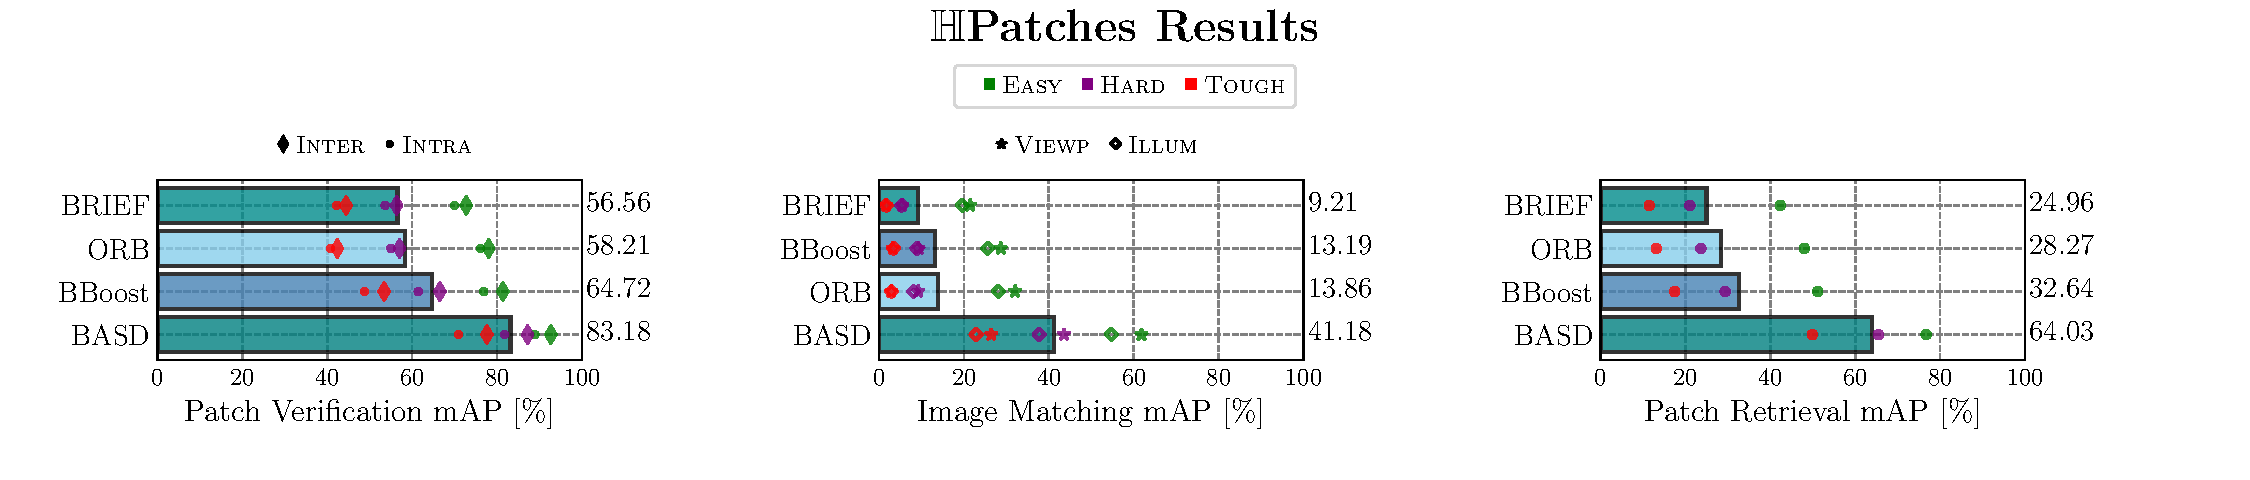
\includegraphics[scale=0.25]{HPatches--orb_brief_binboost_BASD}
\captionsetup{font={scriptsize}}
\caption{The HPatches Results.} \scriptsize
\end{figure}


\subsubsection{Matching result in hard scenarios}
The performance in dealing with hard scenarios like illumination change and view change is very important to SLAM. So we choose the hand-crafted descriptor, ORB, to make a comparison with our learned descriptor. Although we do RANSAC in SLAM system, the performance will be bad if the mismatch number exceeds the match number. We choose large illumination change and large view change pictures to evaluate descriptors. From the match results, our descriptor outperforms the ORB descriptor, which show the robustness of our descriptor.

%\begin{figure}[htbp]
%%\centering
%
%\subfigure[BASD]{
%\begin{minipage}[t]{1\linewidth}
%\centering
%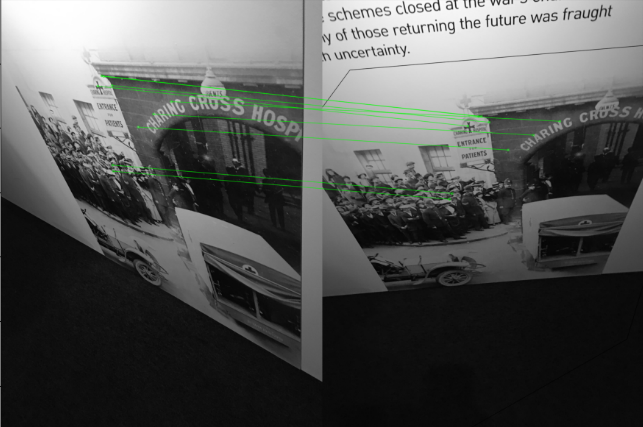
\includegraphics[scale=0.29]{BASD_match.png}
%\end{minipage}
%}
%\subfigure[ORB]{
%\begin{minipage}[t]{1\linewidth}
%\centering
%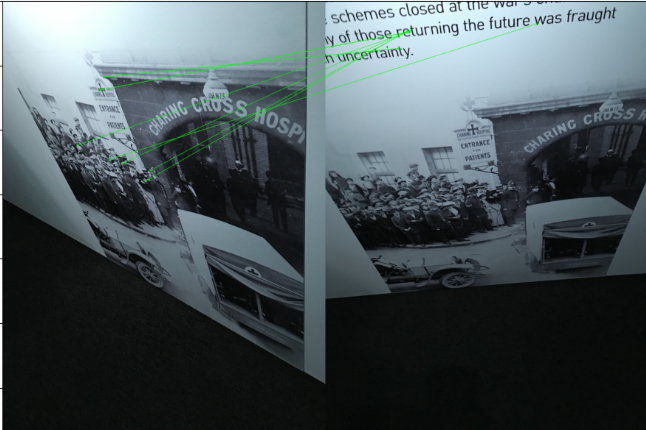
\includegraphics[scale=0.32]{ORB_match.png}
%
%\end{minipage}
%}

%\begin{figure}[htbp]
%\centering
%\begin{minipage}[t]{1\linewidth}
%\centering
%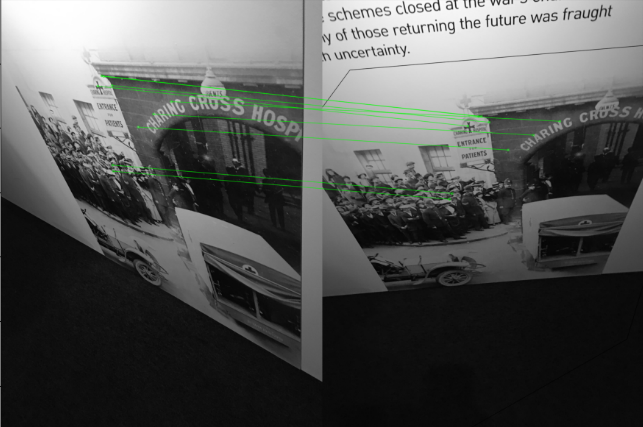
\includegraphics[scale=0.29]{BASD_match.png}
%\label{fig_22}
%\caption{BASD}
%\end{minipage}%
%\begin{minipage}[t]{1\linewidth}
%\centering
%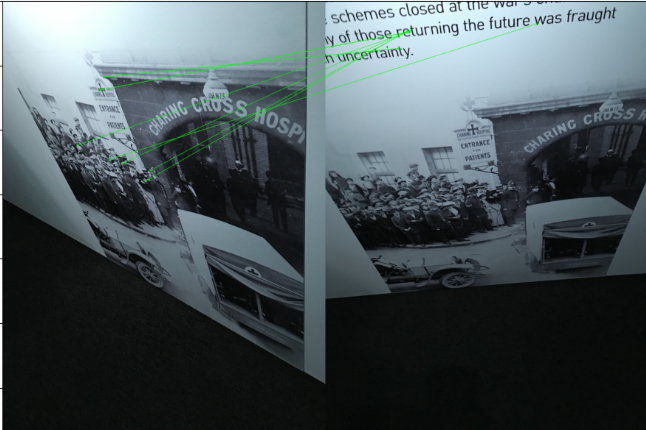
\includegraphics[scale=0.32]{ORB_match.png}
%\caption{ORB}
%\label{fig_23}
%\end{minipage}
%\end{figure}

\begin{figure} 
\centering    
\subfigure[BASD] {
 \label{fig:a}     
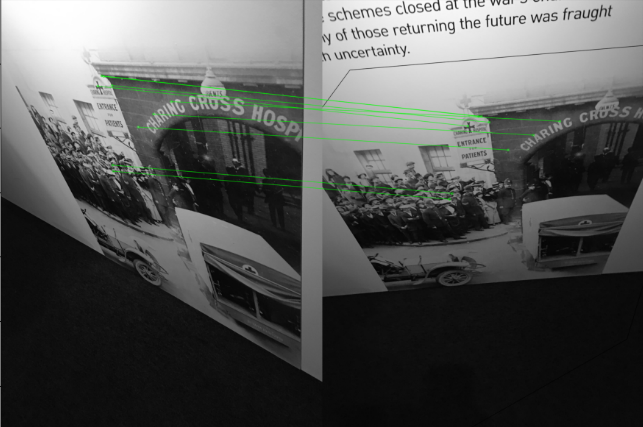
\includegraphics[scale=0.45]{BASD_match.png}  
}     
\subfigure[ORB] { 
\label{fig:b}     
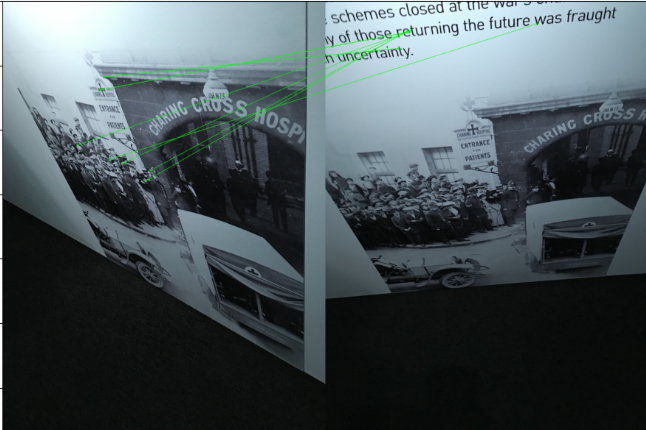
\includegraphics[scale=0.45]{ORB_match.png}     
}      
\caption{ general title. }     
\label{fig}     
\end{figure}

\subsection{SLAM system evaluation}

\subsubsection{Evaluation of KITTI Odometry dataset}
Our descriptors can initialize faster than orb on Kitti, which shows that our descriptors are more robust when the perspective switches quickly.

\subsubsection{Evaluation of Tartanair dataset}
To evaluate the accuracy and robustness of our learned descriptor in BASD-SLAM, we introduce the Tartanair dataset for localization and mapping evaluation. We compared our system with ORB-SLAM2, including the evaluation standard, ATE( absolute trajectory error) and SR(success rate). In order to present the robustness of our descriptor, we respectively choose three contexts in Tartanair, Soul-City, Japanese-Alley, Ocean. The evaluation results are shown in TABLE I. The bold represents the better result. We also choose the evo evaluation tool to estimate and visualize some context trajectory. And the results are shown in TABLE II. From the evaluation results above, we can easily draw the conclusion that our learned descriptor SLAM system outperforms the traditional descriptor SLAM system ORB-SLAM2.

%%%%%%%%%%%%%%%%%%%%%%%%%%%%%%%%%%%%%%%%%%%%%%%%%%%%%%%%%%%%%%%%%%%%%%%%%%%%%%

\section{CONCLUSIONS}

In this paper, we have presented a novel


%%%%%%%%%%%%%%%%%%%%%%%%%%%%%%%%%%%%%%%%%%%%%%%%%%%%%%%%%%%%%%%%%%%%%%%%%%%%%%
\section*{ACKNOWLEDGMENT}

This work is supported by The National Key Research and Development Program of China under Project of 2017YFB0102503 and the National Natural Science Foundation of China under Project of 51605285.



%%%%%%%%%%%%%%%%%%%%%%%%%%%%%%%%%%%%%%%%%%%%%%%%%%%%%%%%%%%%%%%%%%%%%%%%%%%%%%%%

\begin{thebibliography}{99}

\bibitem{c1} Lowe D G . Distinctive Image Features from Scale-Invariant Keypoints[J]. International Journal of Computer Vision, 2004, 60(2):91-110.
\bibitem{c2} Bay H , Ess A , Tuytelaars T , et al. Speeded-Up Robust Features (SURF)[J]. Computer Vision and Image Understanding, 2008, 110(3):346-359.
\bibitem{c3} Rublee E , Rabaud V , Konolige K , et al. ORB: An efficient alternative to SIFT or SURF[C]// 2011 International Conference on Computer Vision. IEEE, 2012.
\bibitem{c4} Mur-Artal R , Montiel J M M , Tardos J D . ORB-SLAM: a Versatile and Accurate Monocular SLAM System[J]. IEEE Transactions on Robotics, 2015, 31(5):1147-1163.
\bibitem{c5} Simo-Serra E , Trulls E , Ferraz L , et al. Discriminative Learning of Deep Convolutional Feature Point Descriptors[C]// 2015 IEEE International Conference on Computer Vision (ICCV). IEEE, 2016.
\bibitem{c6} Tian Y , Fan B , Wu F . L2-Net: Deep Learning of Discriminative Patch Descriptor in Euclidean Space[C]// 2017 IEEE Conference on Computer Vision and Pattern Recognition (CVPR). IEEE, 2017.
\bibitem{c7} A. Mishchuk, D. Mishkin, F. Radenovic, and J. Matas, “Working hard to know your neighbor’s margins: Local descriptor learning loss,” in Advances in Neural Information Processing Systems, 2017, pp. 4826– 4837.
\bibitem{c8} Z. Dai, X. Huang, W. Chen, L. He and H. Zhang, "A Comparison of CNN-Based and Hand-Crafted Keypoint Descriptors," 2019 International Conference on Robotics and Automation (ICRA), Montreal, QC, Canada, 2019, pp. 2399-2404.
\bibitem{c9} J. L. Schönberger, H. Hardmeier, T. Sattler, and M. Pollefeys, ‘‘Comparative evaluation of hand-crafted and learned local features,’’ in Proc. IEEE Conf. Comput. Vis. Pattern Recognit., Jul. 2017, pp. 6959–6968.
\bibitem{c10} J. Wu, Z. Cui, V. S. Sheng, P. Zhao, D. Su, and S. Gong, “A comparative study of sift and its variants,” Measurement science review, vol. 13, no. 3, pp. 122–131, 2013.
\bibitem{c11} Xufeng Han, T. Leung, Y. Jia, R. Sukthankar and A. C. Berg, "MatchNet: Unifying feature and metric learning for patch-based matching," 2015 IEEE Conference on Computer Vision and Pattern Recognition (CVPR), Boston, MA, 2015, pp. 3279-3286.
\bibitem{c12} S. Zagoruyko and N. Komodakis, "Learning to compare image patches via convolutional neural networks," 2015 IEEE Conference on Computer Vision and Pattern Recognition (CVPR), Boston, MA, 2015, pp. 4353-4361.
\bibitem{c13} E. Simo-Serra, E. Trulls, L. Ferraz, I. Kokkinos, P. Fua and F. Moreno-Noguer, "Discriminative Learning of Deep Convolutional Feature Point Descriptors," 2015 IEEE International Conference on Computer Vision (ICCV), Santiago, 2015, pp. 118-126.
\bibitem{c14} Balntas V , Johns E , Tang L , et al. PN-Net: Conjoined Triple Deep Network for Learning Local Image Descriptors[J]. 2016.
\bibitem{c15} V. Balntas, E. Riba, D. Ponsa, and K. Mikolajczyk. Learning local feature descriptors with triplets and shallow convolutional neural networks. Proceedings of the British Machine Vision Conference (BMVC), 2016. 1, 2, 7, 8
\bibitem{c16} F. Schroff, D. Kalenichenko and J. Philbin, "FaceNet: A unified embedding for face recognition and clustering," 2015 IEEE Conference on Computer Vision and Pattern Recognition (CVPR), Boston, MA, 2015, pp. 815-823.
\bibitem{c17} E. Hoffer and N. Ailon. Deep metric learning using Triplet network. International Workshop on Similarity-Based Pattern Recognition, 2015. 2, 3, 10
\bibitem{c18} M. Keller, Z. Chen, F. Maffra, P. Schmuck and M. Chli, "Learning Deep Descriptors with Scale-Aware Triplet Networks," 2018 IEEE/CVF Conference on Computer Vision and Pattern Recognition, Salt Lake City, UT, 2018, pp. 2762-2770.
\bibitem{c19} Yan Ke and R. Sukthankar, "PCA-SIFT: a more distinctive representation for local image descriptors," Proceedings of the 2004 IEEE Computer Society Conference on Computer Vision and Pattern Recognition, 2004. CVPR 2004., Washington, DC, USA, 2004, pp. II-II.
\bibitem{c20} T. Trzcinski, M. Christoudias, P. Fua, and V. Lepetit. Boosting binary keypoint descriptors. In Proceedings of the IEEE conference on computer vision and pattern recognition, pages 2874–2881, 2013.
\bibitem{c21} Y. Gao, W. Huang and Y. Qiao, "Local Multi-Grouped Binary Descriptor With Ring-Based Pooling Configuration and Optimization," in IEEE Transactions on Image Processing, vol. 24, no. 12, pp. 4820-4833, Dec. 2015.
\bibitem{c22} D. DeTone, T. Malisiewicz and A. Rabinovich, "SuperPoint: Self-Supervised Interest Point Detection and Description," 2018 IEEE/CVF Conference on Computer Vision and Pattern Recognition Workshops (CVPRW), Salt Lake City, UT, 2018, pp. 337-33712.
\bibitem{c23} Ono Y , Trulls E , Fua P , et al. LF-Net: Learning Local Features from Images[J]. 2018.
\bibitem{c24} Yi K M , Trulls E , Lepetit V , et al. LIFT: Learned Invariant Feature Transform[J]. 2016.
\bibitem{c25} Bromley J , Guyon I , Lecun Y , et al. Signature Verification Using a Siamese Time Delay Neural Network[C]// Advances in Neural Information Processing Systems 6, [7th NIPS Conference, Denver, Colorado, USA, 1993]. Morgan Kaufmann Publishers Inc. 1993.
\bibitem{c26} E. Hoffer and N. Ailon. Deep metric learning using Triplet network. International Workshop on Similarity-Based Pat- tern Recognition, 2015. 2, 3, 10
\bibitem{c27} S. Wang, R. Clark, H. Wen and N. Trigoni, "DeepVO: Towards end-to-end visual odometry with deep Recurrent Convolutional Neural Networks," 2017 IEEE International Conference on Robotics and Automation (ICRA), Singapore, 2017, pp. 2043-2050.
\bibitem{c28} T. Zhou, M. Brown, N. Snavely and D. G. Lowe, "Unsupervised Learning of Depth and Ego-Motion from Video," 2017 IEEE Conference on Computer Vision and Pattern Recognition (CVPR), Honolulu, HI, 2017, pp. 6612-6619.
\bibitem{c29} C. Zhao, L. Sun, P. Purkait, T. Duckett and R. Stolkin, "Learning Monocular Visual Odometry with Dense 3D Mapping from Dense 3D Flow," 2018 IEEE/RSJ International Conference on Intelligent Robots and Systems (IROS), Madrid, 2018, pp. 6864-6871.
\bibitem{c30} A. Vakhitov and V. Lempitsky, "Learnable Line Segment Descriptor for Visual SLAM," in IEEE Access, vol. 7, pp. 39923-39934, 2019.
\bibitem{c31} C. Yu et al., "DS-SLAM: A Semantic Visual SLAM towards Dynamic Environments," 2018 IEEE/RSJ International Conference on Intelligent Robots and Systems (IROS), Madrid, 2018, pp. 1168-1174.
\bibitem{c32} N. Brasch, A. Bozic, J. Lallemand and F. Tombari, "Semantic Monocular SLAM for Highly Dynamic Environments," 2018 IEEE/RSJ International Conference on Intelligent Robots and Systems (IROS), Madrid, 2018, pp. 393-400.
\bibitem{c33} T. Naseer, G. L. Oliveira, T. Brox and W. Burgard, "Semantics-aware visual localization under challenging perceptual conditions," 2017 IEEE International Conference on Robotics and Automation (ICRA), Singapore, 2017, pp. 2614-2620.
\bibitem{c34} A. Loquercio, M. Dymczyk, B. Zeisl, S. Lynen, I. Gilitschenski and R. Siegwart, "Efficient descriptor learning for large scale localization," 2017 IEEE International Conference on Robotics and Automation (ICRA), Singapore, 2017, pp. 3170-3177.
\bibitem{c35} Z. Zhang and D. Scaramuzza, "A Tutorial on Quantitative Trajectory Evaluation for Visual(-Inertial) Odometry," 2018 IEEE/RSJ International Conference on Intelligent Robots and Systems (IROS), Madrid, 2018, pp. 7244-7251.
\bibitem{c36} X. Gao, R. Wang, N. Demmel and D. Cremers, "LDSO: Direct Sparse Odometry with Loop Closure," 2018 IEEE/RSJ International Conference on Intelligent Robots and Systems (IROS), Madrid, 2018, pp. 2198-2204.
\end{thebibliography}




\end{document}
